\documentclass[]{scrartcl}
\usepackage{Preamble}

\setcounter{section}{4}
\newcommand{\exercise}{Exercise \thesection}
\newcommand{\duedate}{2020-12-14, 23:59}

\begin{document}
\section*{\exercise}

To compile: unzip our uploaded code, and run \verb|make| inside \verb|code/|.
The slurm scripts are stored inside \verb|code/slurm/|.
To debug: run the debug outputs (\verb|*.dbg|) and attach gdb to respective pids

\subsection{Reading}
\subsection{Matrix multiply --- parallel version using MPI}
\subsection{Matrix multiply --- scaling process count}
\begin{table}[ht]
    \centering
    \begin{tabular}{rr}
\toprule
 nodes &  GFLOPS64/s \\
\midrule
     1 &     1.55161 \\
     3 &     2.28341 \\
     5 &     2.89719 \\
     7 &     3.89113 \\
     9 &     4.90389 \\
    11 &     5.42166 \\
    13 &     6.30550 \\
    15 &     7.30316 \\
\bottomrule
\end{tabular}

\end{table}
\begin{figure}[ht]
    \centering
    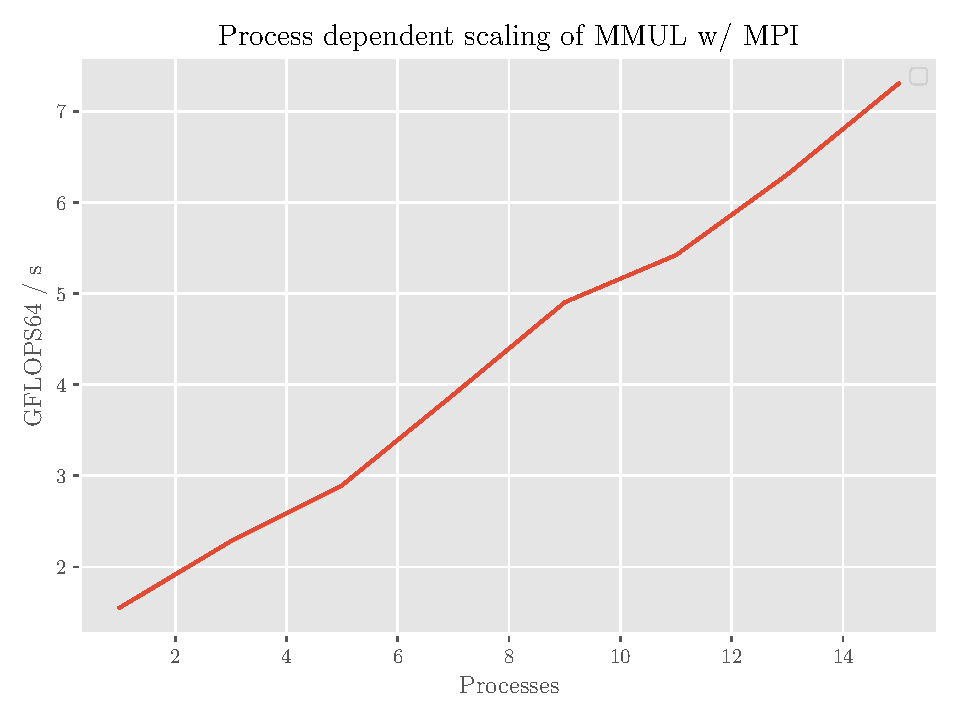
\includegraphics[width=\linewidth]{img/scaling_proc.pdf}
    \caption{Scaling Process Count}%
    \label{fig:scaling_proc}
\end{figure}
\subsection{Matrix multiply --- scaling problem size}

feqw

\end{document}
